\documentclass[10pt,a4j]{jsarticle}
\usepackage{amsmath}
\usepackage[dvipdfmx]{graphicx}
\usepackage{url}
\usepackage{here}
% プリアンブル

\makeatletter
\newcommand{\subsubsubsection}{\@startsection{paragraph}{4}{\z@}%
  {1.0\Cvs \@plus.5\Cdp \@minus.2\Cdp}%
  {.1\Cvs \@plus.3\Cdp}%
  {\reset@font\sffamily\normalsize}
}
\makeatother
\setcounter{secnumdepth}{4}
\title{\vspace{-2.5cm}金属材料の組織観察と引張試験}
\author{1610581 堀田 大地}
\date{2018/5/31}
\begin{document}
\maketitle{}
\section{目的}
% 目的
焼きなまし焼き入れ,焼き入れ焼き戻しの熱処理を施した各種炭素鋼の金属組織を光学顕微鏡で観察し,
熱処理による組織の変化を学ぶ.
また,炭素鋼とアルミニウム合金を用いて引張試験を行い,
応力ーひずみ線図を作成して引張試験から得られる機械的特性について学ぶ.
% 実験
\section{金属材料の組織観察}
% 金属材料の組織観察
  \subsection{目的}
  % 目的
  機械材料の性質判定の手段として,古くから光学顕微鏡による組織観察が用いられてきたが,禁煙は走査型電子顕微鏡,透過型電子顕微鏡による組織観察が用いられており,組織と金属材料の特性との研究がされている.
  そこで,炭素鋼を資料として用いて,焼なまし,焼入れ,焼入れ焼もどしの熱処理を施した試料表面の組織を観察し,
  組織の種類,配置分布,形状,大きさとこれらの相互関係を調べると共に,熱処理による組織の変化について学ぶことを
  目的とする.
  \subsection{Fe-Cの平衡状態図と熱処理}
  熱処理には焼なまし,焼ならし,焼入れ,焼もどしがある.
  焼なましとは,鋼を均一オーステナイト状態まで加熱・保持した後,炉内でゆっくり冷却する熱処理であり,この時得られる
  組織を標準組織と言う.標準組織の鉄鋼は次式で与えられる引張り強さ$σ_{B}$で示すことが知られている.
    \begin{center}
	  $σ_{B} =281 \times (1-\frac{C\%}{0.8})+830 \times (\frac{C\%}{0.8})  (MPa)
      $\quad(1)
  \end{center}
  焼ならしは,焼なまし処理と同様に鉄鋼を均一オーステナイト状態まで加熱・保持した後,
  空気中で自然冷却する熱処理で,その結果得られる組織をソルバイトと呼び,強さと
  靭性の優れた鉄鋼材が得られる.
  しかし,焼ならしでは機械構造用部品等に要求される強さと靭性は十分得られな場合があり,この場合に焼入れと焼もどしを行う.
  焼入れは,鉄鋼を均一オーステナイト状態まで加熱・保持した後,水中または油中に炭素鋼を入れて急冷する熱処理であり,
  オーステナイトが無拡散変態によりマルテンサイトに変態する.
  焼もどしは,焼入れの後に再加熱し,冷却する熱処理で,鉄鋼はソルバイトまたはトルースタイトの組織になる.
  
  \subsection{試料作成と検鏡法}
  	% 試料作成と検鏡法
    \subsubsection{試料}
    % 試料
    表1に今回用いた試料を示した
    \begin{table}[H]
      \centering
      \caption{組織観察用の資料の種類}
        \label{my-label}
        \footnotesize
        \begin{tabular}{l|lll}
                    & No. & 熱処理     &                    \\ \hline
          極軟鋼        & 22  & 焼なまし    & 焼きなまし              \\
          S15C       & 23  & 焼なまし    & 極軟鋼:950℃30分加熱→炉冷   \\
          S45C       & 24  & 焼なまし    & S15C:900℃30分加熱→炉冷  \\
                    & 25  & 焼入れ     & S45C:850℃60分加熱→炉冷  \\
                    & 26  & 焼入れ焼もどし & SK105:850℃60分加熱→炉冷 \\
          S85(SK5)   & 27  & 焼なまし    & SK85:950℃60分加熱→炉冷  \\
                    & 28  & 焼入れ     & 焼入れ                \\
                    & 29  & 焼入れ焼もどし & 850℃30分加熱→水焼入れ     \\
          SK105(SK3) & 30  & 焼なまし    & 焼もどし               \\
                    & 31  & 焼入れ     & 焼入れ後,600℃30分加熱→空冷  \\
                    & 32  & 焼入れ焼もどし &                   
        \end{tabular}
      \end{table}
    \subsubsection{研磨}
    % 研磨
    顕微鏡資料の作成は以下の手順で行った.
    \begin{enumerate}
      \item 試料の選定 \\
      \item エメリー紙研磨\#1000で一方向のみへの研磨.次に\#1500で試料を$\frac{\pi}{2}$回転させて
      研磨. \\
      \item さらに試料を$\frac{\pi}{2}$回転させ酸化クロム(I\hspace{-.1em}I\hspace{-.1em}I)
      で仕上げ研磨(バフ研磨) \\
    \end{enumerate}
    \subsubsection{エッチング}
    % エッチング
    光学顕微鏡で,主に試料面の凹凸の差により起こる反射光の明暗の差によって組織を調べるため,適当な
    腐蝕液で腐蝕する必要があるので,表2に示す腐蝕液で腐蝕を行なった. 
    試料表面を腐蝕液に浸し,適切な腐蝕時間経過後,直ちに試料表面を流水で洗い流し
    乾燥させた.
    \begin{table}[H]
      \centering
      \caption{エッチング}
      \label{my-label}
      \footnotesize
      \begin{tabular}{llllll}
        金属名 & No.        & エッチング液(腐蝕液)        & 時間 & 適用          \\ \hline
        鉄鋼  & 22$\sim$30 & 硝酸アルコール(Nital)      & 数秒$\sim$60秒 & 炭素鋼のすべての組織,パーライトは黒く着色,フェライト粒界隈が現出する. \\
            & 31,32      & ピクリン酸アルコール(Picral) & 数秒$\sim$60秒 & 炭素鋼のすべての組織.
      \end{tabular}
    \end{table}
    \subsubsection{検鏡}
    % 検鏡
    金属顕微鏡は,試料面に対して垂直に光を当てて反射光によって観察を行うので,
    光軸に対して試料面を垂直におく必要があるので,試料をスライドガラス上に
    付着させた油粘土の上に載せて,試料平圧器を用いて,上から静かに押して
    試料面がスライドガラス面と平衡になるようにした.
    このスライドガラスに固定された試料を顕微鏡のステージに載せて検鏡した.

  
\section{金属材料の引張試験}
% 金属材料の引張試験
  \subsection{目的}
  % 目的
  機械,構造物の設計に必要な金属材料の性的な機械的特性を取得するためには,金属材料の引張試験を行う必要がある.
  この試験により,金属材料の弾性と塑性の特性,引張強さ,破断伸び,破断絞りなどの基本的な機械的特性を測定
  することができるので,炭素鋼とアルミニウム合金を供試材として,引張試験を行い,機械的特性を測定し,
  引張試験方法を習得すると共に,炭素鋼とアルミニウム合金の機械特性の違いについて学ぶことを目的とする.
  \subsubsection{引張試験}
  % 引張試験
  引張試験は,試験片に引張荷重を加え,破断に至るまでひずみを与え,金属材料の縦弾性係数,
  降伏点,0.2\%耐力,引張強さ,破断伸び,破断絞りなどの機械的特性を測定する試験である.
  程炭素鋼の応力ーひずみ線図において,上降伏点より手前では,応力とひずみの間に比例関係があり,
  その傾きを縦弾性係数(ヤング率),この範囲を弾性行きと呼び,応力を$0$に戻せばひずみも
  $0$に戻る.この点に応力が達すると材料が降伏を開始する.この点以降は,塑性域と呼ぶ.
  降伏領域を過ぎると,加工硬化によって材料の変形抵抗が増加し,最大応力点に達する.
  その後,試験片平行部でくびれが生じ始めるため,応力が返照し最後に試験片が破断する.
  また,非鉄金属の応力ーひずみ線図では,明瞭な降伏点は現れいので,0.2\%の塑性ひずみ
  が生ずる応力を0.2\%耐力と呼び,降伏点の代わりに用いる.
  \subsubsection{試験装置}
  % 試験装置
  コンピュータ制御型万能試験機(Istron社製 4505)を用いた.
  本装置は,試験装置本体,制御装置,PCから構成された.
  \subsubsection{供試材}
  % 供試材
  A1100(アルミニウム合金)と900℃,1時間で焼なまししたSPCC(冷間圧延鋼板)を用いた.
  \subsubsection{縦弾性係数(ヤング率)の測定}
  % 縦弾性係数(ヤング率)の測定
  供試材の縦弾性係数を求めるために,試験片評点間の中央付近にひずみゲージを専用の接着剤
  を用いて貼った.ひずみゲージは,共和電業製,ベース長$9.4mm$,ベース幅$2.8mm$,
  グリッド長$5mm$,グリッド幅$1.4mm$のKFG-5-120-C1を用いた.
  ひずみゲージとは,試験片の評点部の「ひずみ」を電気信号として検出するセンサーである.
  \subsubsection{引張試験手順}
  % 引張試験手順
  \begin{enumerate}
    \item 各試験片の平行部の板幅$W_{0}$と板厚$B_{0}$を数カ所測定し,それらの平均値を用いて
    原断面積$A_{0}$(初期断面積)を求めた.
    次に,破断伸びを測定するために試験片平行部に
    票点距離$L_{0}$が$50mm$になるように2本の線を書き破断伸びを測定する基準とした.
    $W_{0}$,$B_{0}$,$L_{0}$を3回ずつ測定し,表3,4に示した.\\
    \item 試験片の上部の掴み部を試験機のチャックに取り付けた. \\
    \item ひずみゲージの配線を行なった. \\
    \item 試験片の下部の掴み部を試験機のチャックに取り付けた.その際,
    引張荷重,圧縮荷重が付加されないように試験機のクロスヘッドを微動させながら,
    チャックに取り付けた. \\
    \item クロスヘッド速度$1.0mm/min$で,引張試験を行なった.
    引張試験で,荷重$P$,クロスヘッドの変位$L$,ひずみゲージから求めたひずみ$ε$
    を2台のPCで測定した. \\
    \item 引張試験終了後,破断部の板幅$W_{f}$,板厚$B_{f}$を数カ所3回測定した.
    また,それらの平均値を用いて破断部の断面積$A_{f}$を求めた.さらに,試験片の破断面
    を付合わせて破断後の評点間距離$L_{f}$を求めた.これらの表5,6に示した. \\
    \item 荷重$P$ー変位$L$の関係から,公称応力$σ$ー公称ひずみ$ε$線図を書き
    上降伏点,下降伏点,引張強さを求めた.また真応力$σ_{t}$ー真ひずみ$ε_{t}$線図を作成した.
    破断伸び,破断絞りを求めた.\\
    \item 式(9)を用いて公称ひずみ$ε$から真ひずみ$ε_{t}$を計算した.
    真応力$σ_{t}$は,最大応力までは式(7)を用いて公称応力$σ$と公称ひずみ$ε$から計算した.
    最大応力以降は試験片にくびれが発生するため式(6)が成立しないので,破断時の荷重$P_{f}$と
    破断部の断面積$A_{f}$から破断時の真応力$σ_{tf}$をプロットした.式(7)から求めた最大応力
    までの真応力$σ_{t}$と破断時の真応力$σ_{tf}$の間は,フリーハンドで書いた.\\
    \item ひずみケージから求めたひずみ$ε$を用いて,公称応力$σ$ー公称ひずみ$ε$線図を作成し,
    縦弾性係数の計算を行なった.また,A1100の場合,0.2\%耐力もこの図から求めた.
    \item 機械特性を求めるための計算式は次の通りである.
      \begin{enumerate}
        \item 公称応力$σ$ \\
          $σ = \frac{P}{A_{0}}$\quad(2)
        \item 公称ひずみ$ε$ \\
          $ε = \frac{L-L_{0}}{L_{0}}$\quad(3)
        \item 破断伸び$δ$ \\
          $δ = \frac{L_{f} - L_{0}}{L_{0}} \times 100 (\%)$\quad(4)
        \item 破断絞り$φ$ \\
          $φ = \frac{A_{0} - A_{f}}{A_{0}} \times 100 (\%)$\quad(5)
        \item 真応力$σ_{t}$ \\
          $A_{0}L_{0} = AL$\quad(6) \\
          $σ_{t} = \frac{P}{A} = \frac{P}{A_{0}} \frac{L}{L_{0}} = σ(1+ε)$\quad(7) \\
        \item 真ひずみ$ε_{t}$ \\
          $dε = \frac{dl}{l}$\quad(8) \\
          $ε_{t} = \int_{L_{0}}^{L} \frac{dl}{l}dl = \log \frac{L}{L_{0}} = \log (1+\frac{L-L_{0}}{L_{0}}) = \log (1+ε)$ \quad(9)
      \end{enumerate}
  \end{enumerate}
\section{結果}
% 結果
  \subsection{金属材料の組織観察}
  % 金属材料の組織観察
  顕微鏡での観察結果を図1\~22に示した.
  % gokunankou
  \begin{figure}[htbp]  
    \begin{minipage}{0.5\hsize}
      \begin{center}
        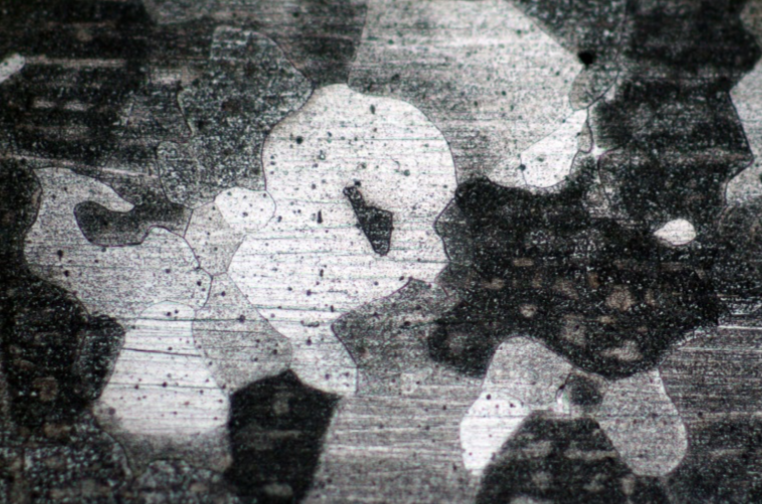
\includegraphics[width=7cm]{../img/gokunankou_yakinamashi_200.png}
        \caption{極軟鋼 焼なまし 倍率:200}
      \end{center}
    \end{minipage}
    \begin{minipage}{0.5\hsize}
      \begin{center}
        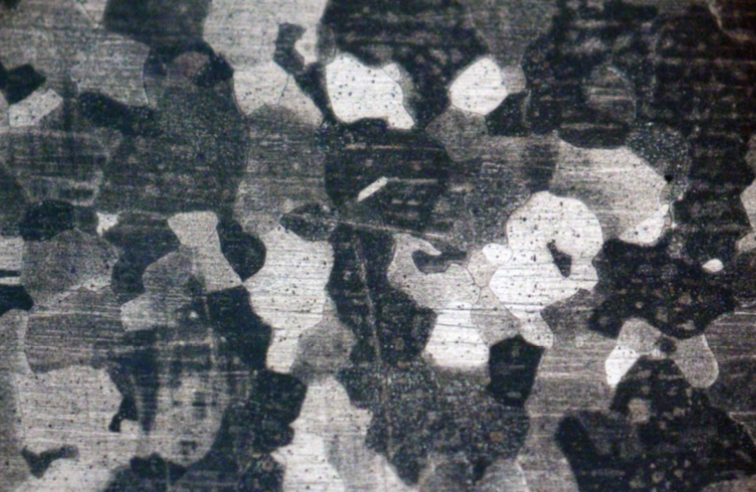
\includegraphics[width=7cm]{../img/gokunankou_yakinamashi_100.png}
        \caption{極軟鋼 焼なまし 倍率:100}
      \end{center}
    \end{minipage}
  \end{figure}
  % S15C
  \begin{figure}[htbp]
    \begin{minipage}{0.5\hsize}
      \begin{center}
        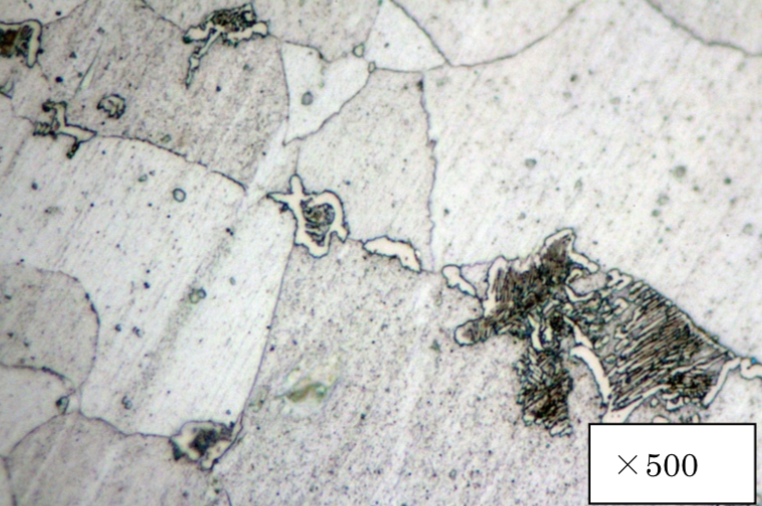
\includegraphics[width=7cm]{../img/S15C_yakinamashi_500.png}
        \caption{S15C 焼なまし 倍率:1000}
      \end{center}
    \end{minipage}
    \begin{minipage}{0.5\hsize}
      \begin{center}
        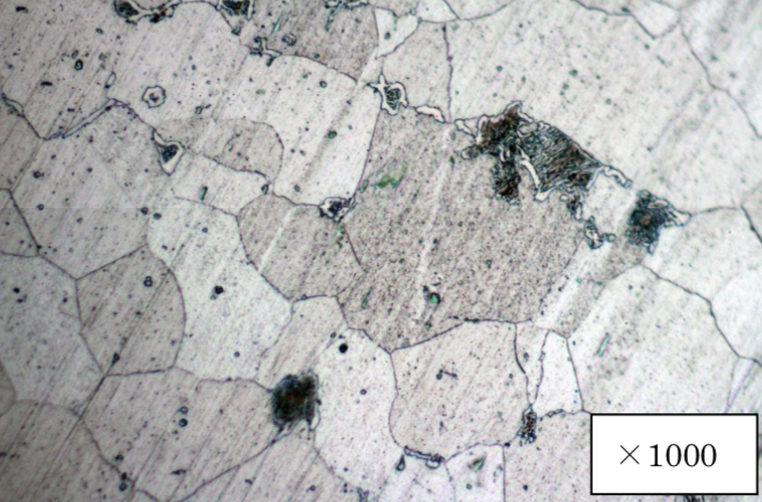
\includegraphics[width=7cm]{../img/S15C_yakinamashi_1000.png}
        \caption{S15C 焼なまし 倍率:500}
      \end{center}
    \end{minipage}
  \end{figure}
  % S45C
  % 焼入れ
  \begin{figure}[htbp]
    \begin{minipage}{0.5\hsize}
      \begin{center}
        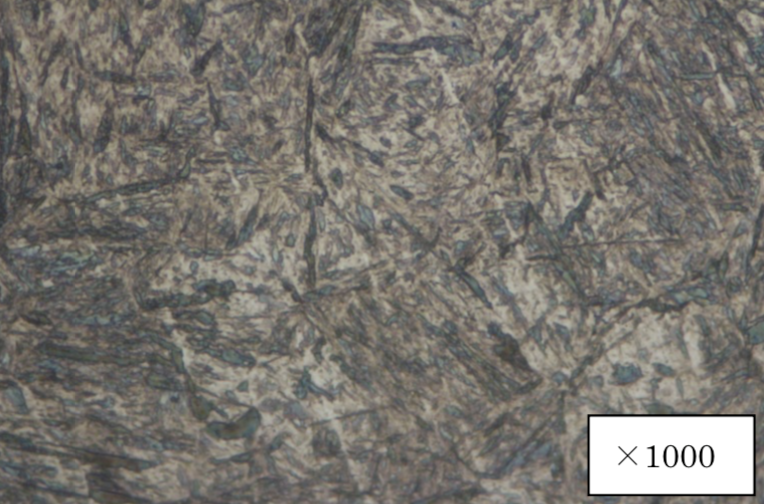
\includegraphics[width=7cm]{../img/S45C_yakiire_1000.png}
        \caption{S45C 焼入れ 倍率:1000}
      \end{center}
    \end{minipage}
    \begin{minipage}{0.5\hsize}
      \begin{center}
        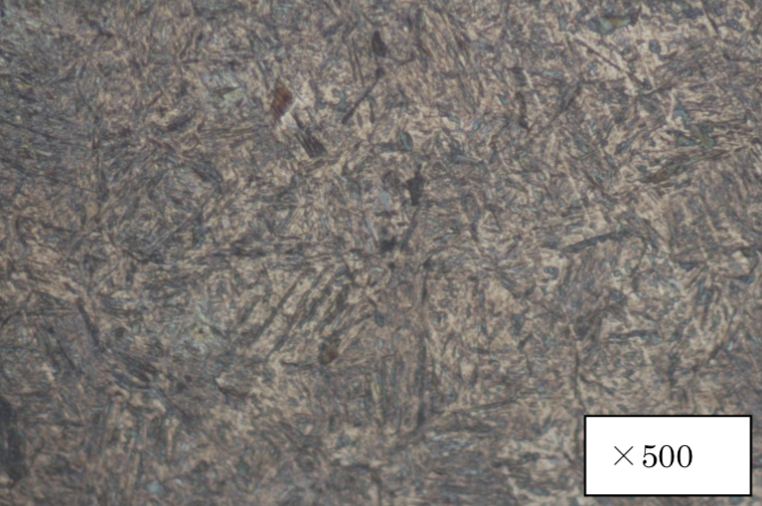
\includegraphics[width=7cm]{../img/S45C_yakiire_500.png}
        \caption{S45C 焼入れ 倍率:500}
      \end{center}
    \end{minipage}
  \end{figure}
  % 焼なまし
  \begin{figure}[htbp]
    \begin{minipage}{0.5\hsize}
      \begin{center}
        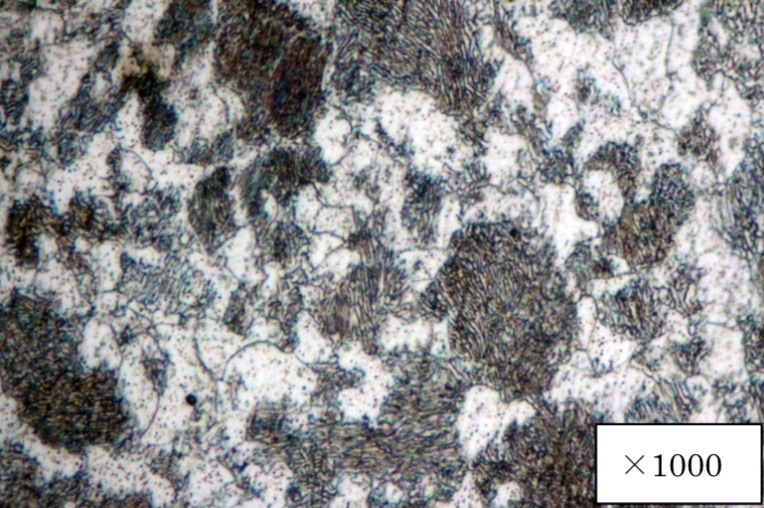
\includegraphics[width=7cm]{../img/S45C_yakinamashi_1000.png}
        \caption{S45C 焼なまし 倍率:1000}
      \end{center}
    \end{minipage}
    \begin{minipage}{0.5\hsize}
      \begin{center}
        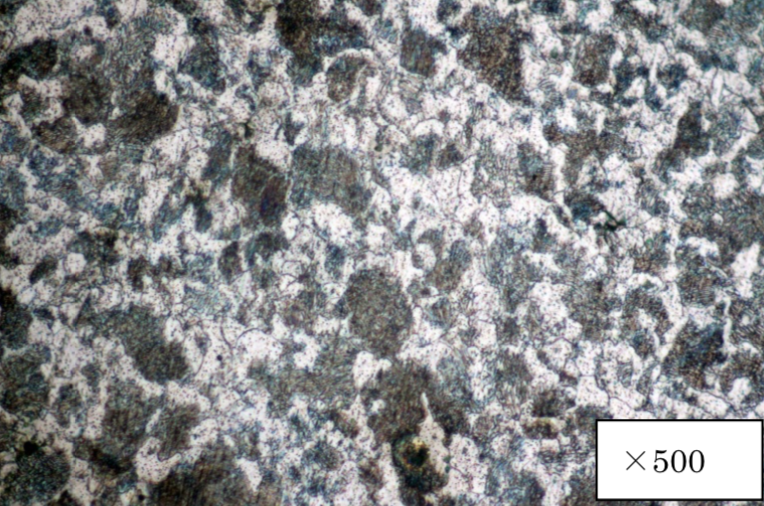
\includegraphics[width=7cm]{../img/S45C_yakinamashi_500.png}
        \caption{S45C 焼なまし 倍率:500}
      \end{center}
    \end{minipage}
  \end{figure}
  % 焼入れ焼戻し
  \begin{figure}[htbp]
    \begin{minipage}{0.5\hsize}
      \begin{center}
        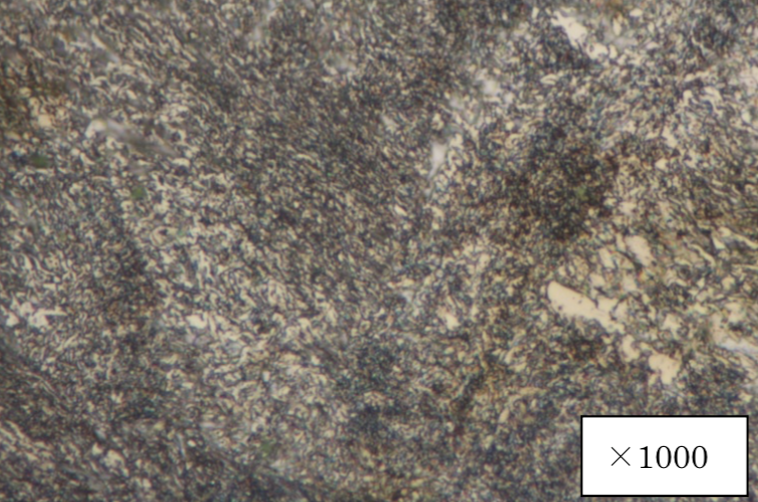
\includegraphics[width=7cm]{../img/S45C_yakiiremodoshi_1000.png}
        \caption{S45C 焼入れ焼きもどし 倍率:1000}
      \end{center}
    \end{minipage}
    \begin{minipage}{0.5\hsize}
      \begin{center}
        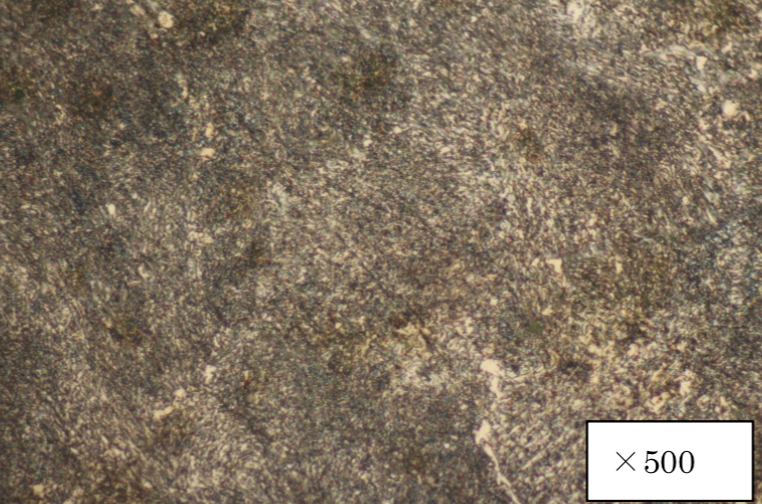
\includegraphics[width=7cm]{../img/S45C_yakiiremodoshi_500.png}
        \caption{S45C 焼入れ焼きもどし 倍率:500}
      \end{center}
    \end{minipage}
  \end{figure}
  % SK85
  % 焼入れ
  \begin{figure}[htbp]
    \begin{minipage}{0.5\hsize}
      \begin{center}
        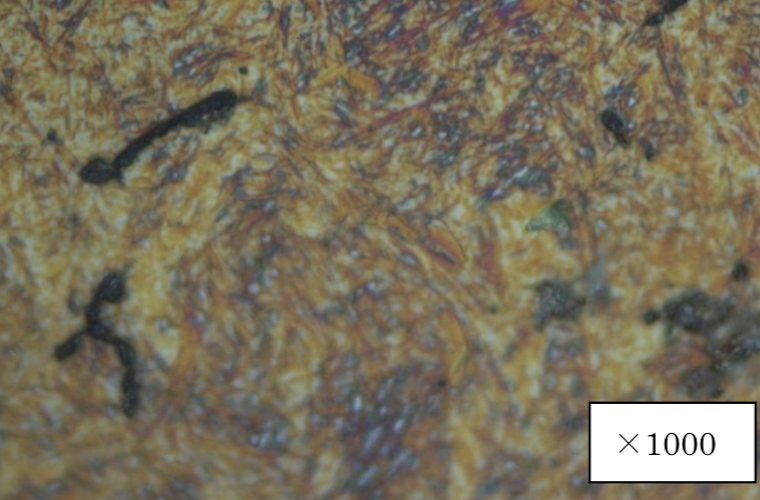
\includegraphics[width=7cm]{../img/SK85_yakiire_1000.png}
        \caption{SK85 焼入れ 倍率:1000}
      \end{center}
    \end{minipage}
    \begin{minipage}{0.5\hsize}
      \begin{center}
        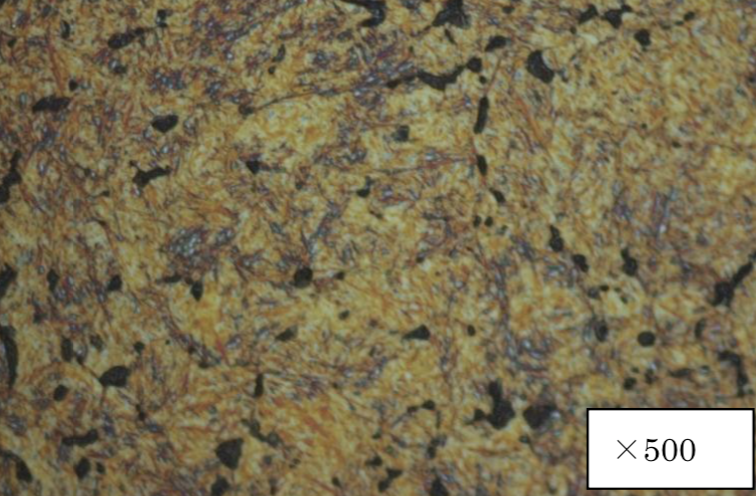
\includegraphics[width=7cm]{../img/SK85_yakiire_500.png}
        \caption{SK85 焼入れ 倍率:500}
      \end{center}
    \end{minipage}
  \end{figure}
  % 焼なまし
  \begin{figure}[htbp]
    \begin{minipage}{0.5\hsize}
      \begin{center}
        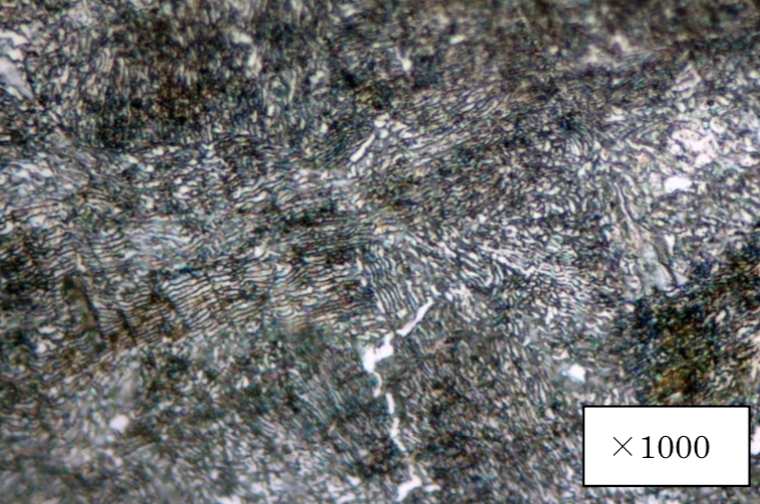
\includegraphics[width=7cm]{../img/S85_yakinamashi_1000.png}
        \caption{SK85 焼なまし 倍率:1000}
      \end{center}
    \end{minipage}
    \begin{minipage}{0.5\hsize}
      \begin{center}
        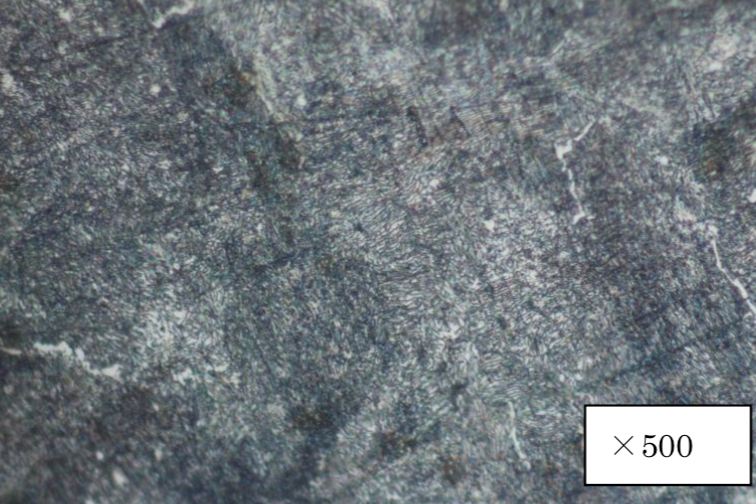
\includegraphics[width=7cm]{../img/SK85_yakinamashi_500.png}
        \caption{SK85 焼なまし 倍率:500}
      \end{center}
    \end{minipage}
  \end{figure}
  % 焼入れ焼もどし
  \begin{figure}[htbp]
    \begin{minipage}{0.5\hsize}
      \begin{center}
        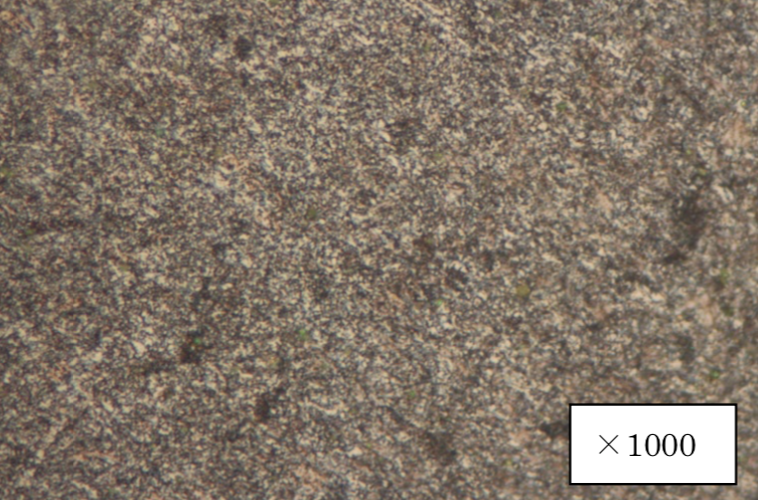
\includegraphics[width=7cm]{../img/SK85_yakiiremodoshi_1000.png}
        \caption{SK85 焼入れ焼きもどし 倍率:1000}
      \end{center}
    \end{minipage}
    \begin{minipage}{0.5\hsize}
      \begin{center}
        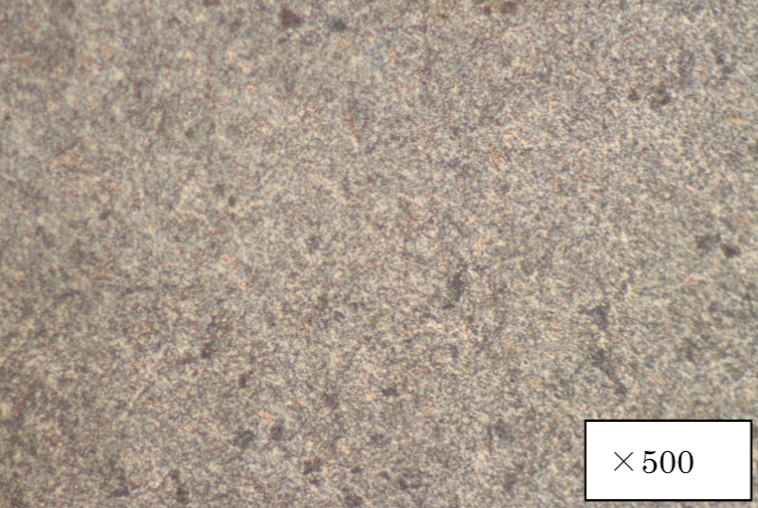
\includegraphics[width=7cm]{../img/SK85_yakiiremodoshi_500.png}
        \caption{SK85 焼入れ焼きもどし 倍率:500}
      \end{center}
    \end{minipage}
  \end{figure}
  % SK105
  % 焼入れ
  \begin{figure}[htbp]
    \begin{minipage}{0.5\hsize}
      \begin{center}
        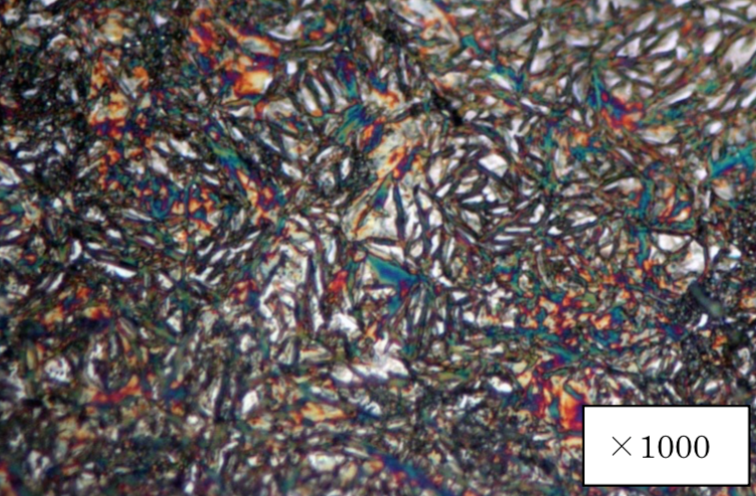
\includegraphics[width=7cm]{../img/SK105_yakiire_1000.png}
        \caption{SK105 焼入れ 倍率:1000}
      \end{center}
    \end{minipage}
    \begin{minipage}{0.5\hsize}
      \begin{center}
        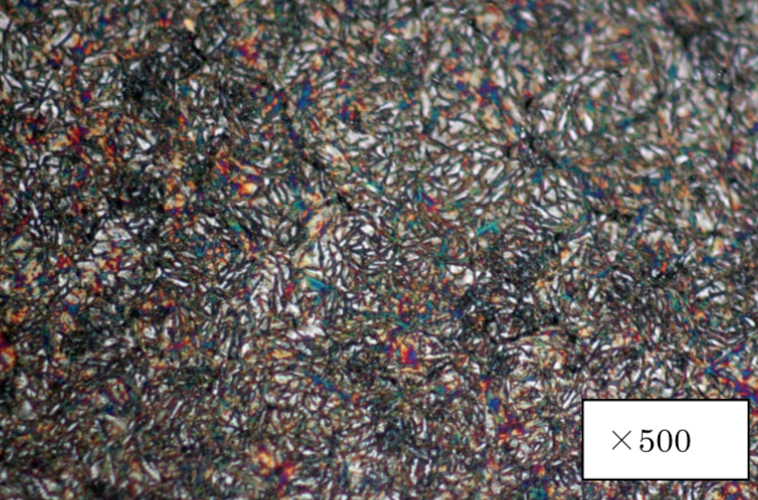
\includegraphics[width=7cm]{../img/SK105_yakiire_500.png}
        \caption{SK105 焼入れ 倍率:500}
      \end{center}
    \end{minipage}
  \end{figure}
  % 焼なまし
  \begin{figure}[htbp]
    \begin{minipage}{0.5\hsize}
      \begin{center}
        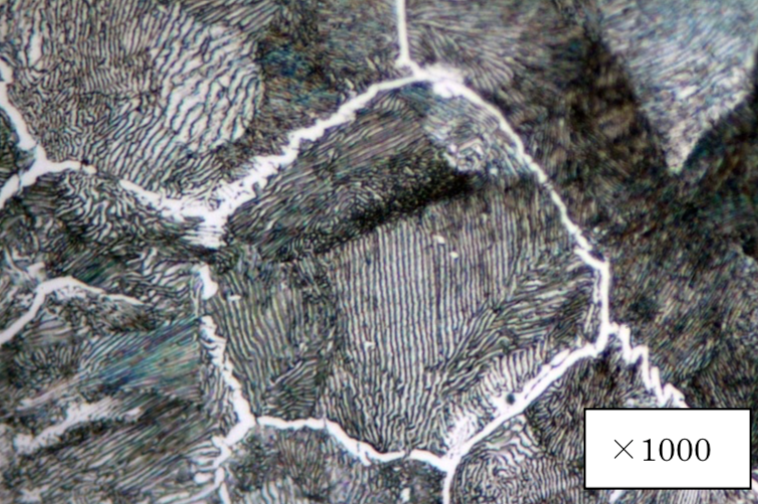
\includegraphics[width=7cm]{../img/SK105_yakinamashi_1000.png}
        \caption{SK105 焼なまし 倍率:1000}
      \end{center}
    \end{minipage}
    \begin{minipage}{0.5\hsize}
      \begin{center}
        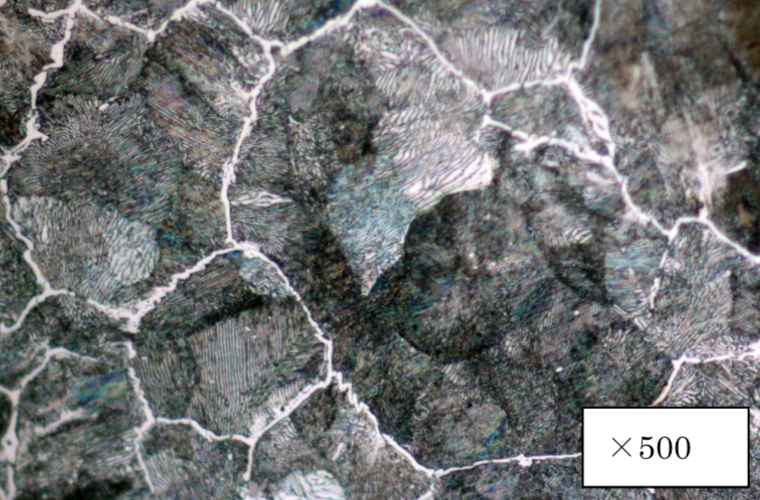
\includegraphics[width=7cm]{../img/SK105_yakinamashi_500.png}
        \caption{SK105 焼なまし 倍率:500}
      \end{center}
    \end{minipage}
  \end{figure}
  % 焼入れ焼もどし
  \begin{figure}[htbp]
    \begin{minipage}{0.5\hsize}
      \begin{center}
        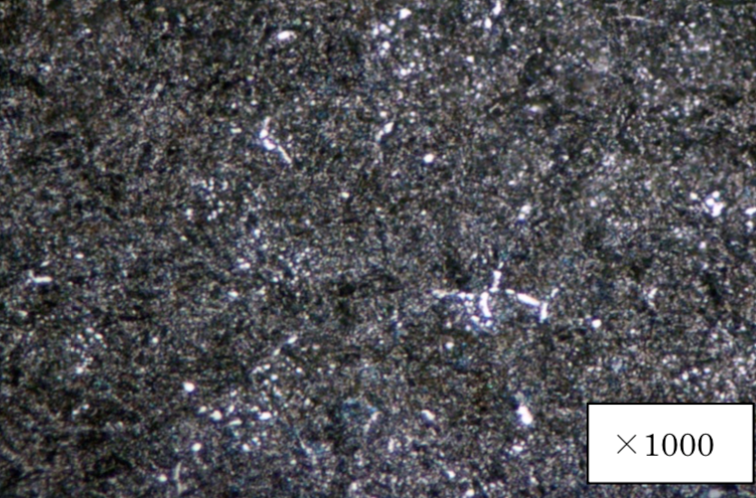
\includegraphics[width=7cm]{../img/SK105_yakiiremodoshi_1000.png}
        \caption{SK105 焼入れ焼きもどし 倍率:1000}
      \end{center}
    \end{minipage}
    \begin{minipage}{0.5\hsize}
      \begin{center}
        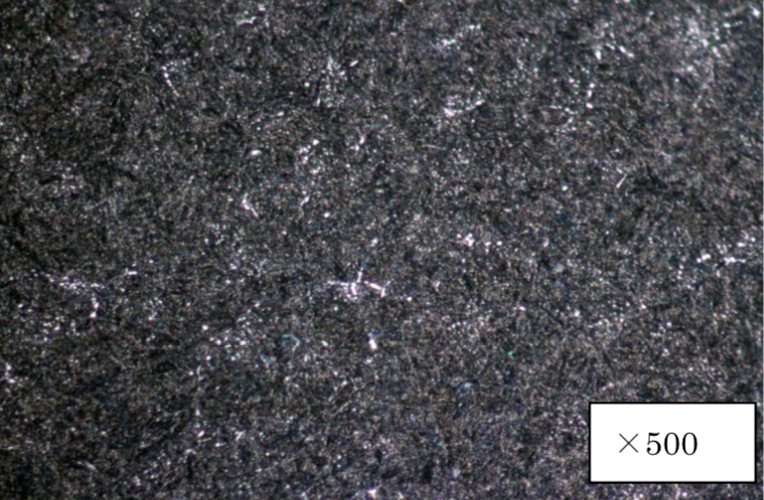
\includegraphics[width=7cm]{../img/SK105_yakiiremodoshi_500.png}
        \caption{SK105 焼入れ焼きもどし 倍率:500}
      \end{center}
    \end{minipage}
  \end{figure}
  \subsection{金属材料の引張試験}
  % 金属材料の引張試験
  \subsubsection{引張試験前の試験片の各種測定結果}
    試験開始前,開始後のSPCC,A1100の寸法を表3,4に示した.
    % 表3
    \begin{table}[H]
      \centering
      \caption{試験開始前のSPCCの寸法}
      \label{my-label}
        \footnotesize
        \begin{tabular}{lllll}
                      & 1回目(mm) & 2回目(mm) & 3回目(mm) & 平均(mm) \\ \hline
        板幅 $W_{0}$    & 12.10   & 12.00   & 12.10   & 12.07  \\
        板厚 $B_{0}$    & 1.790   & 1.785   & 1.795   & 1.79   \\
        断面積 $A_{0}$   & 21.66   & 21.42   & 21.72   & 21.61$mm^{2}$  \\
        標点間距離 $L_{0}$ & 51.0    & 50.5    & 51.0    & 50.83 
      \end{tabular}
    \end{table}
    % 表4
    \begin{table}[H]
      \centering
      \caption{試験開始前のA1100の寸法}
      \label{my-label}
      \footnotesize
      \begin{tabular}{lllll}
                      & 1回目($mm$) & 2回目($mm$) & 3回目($mm$) & 平均($mm$) \\ \hline
        板幅 $W_{0}$    & 12.30   & 12.20   & 12.20   & 12.23  \\
        板厚 $B_{0}$    & 1.985   & 1.990   & 1.980   & 1.985  \\
        断面積 $A_{0}$   & 24.42   & 24.28   & 24.16   & 24.28$mm^{2}$  \\
        標点間距離 $L_{0}$ & 51.00   & 51.50   & 51.00   & 51.17 
      \end{tabular}
    \end{table}
  \subsubsection{引張試験後の試験片の各種測定結果}
    試験開始後の寸法を表5,6に示した.
    % 表5
    \begin{table}[H]
      \centering
      \caption{試験開始後のSPCCの寸法}
      \label{my-label}
        \footnotesize
        \begin{tabular}{lllll}
                      & 1回目($mm$) & 2回目($mm$) & 3回目($mm$) & 平均($mm$) \\ \hline
        板幅 $W_{f}$    & 5.90   & 6.00   & 6.10   & 6.00  \\
        板厚 $B_{f}$    & 0.75   & 0.80   & 0.85   & 0.80   \\
        断面積 $A_{f}$   & 4.43   & 4.80   & 5.12   & 4.80$mm^{2}$  \\
        標点間距離 $L_{f}$ & 73.50    & 73.50    & 73.50    & 73.50 
      \end{tabular}
    \end{table}
     % 表6
    \begin{table}[H]
      \centering
      \caption{試験開始後のA1100の寸法}
      \label{my-label}
        \footnotesize
        \begin{tabular}{lllll}
                      & 1回目($mm$) & 2回目($mm$) & 3回目($mm$) & 平均($mm$) \\ \hline
        板幅 $W_{f}$    & 9.40   & 9.50   & 9.55   & 9.48  \\
        板厚 $B_{f}$    & 0.75   & 0.70   & 0.75   & 0.73   \\
        断面積 $A_{f}$   & 7.05   & 6.65   & 7.16   & 6.92($mm^{2}$)  \\
        標点間距離 $L_{f}$ & 53.5    & 55.0    & 53.5    & 54.0
      \end{tabular}
    \end{table}
  \subsubsection{公称応力―公称ひずみ線図,真応力―真ひずみ線図}
  % 公称応力―公称ひずみ線図,真応力―真ひずみ線図
    それぞれの結果を図23,24に示した.
    \begin{figure}[htbp]
      % 図23
      \begin{minipage}{0.5\hsize}
        \begin{center}
          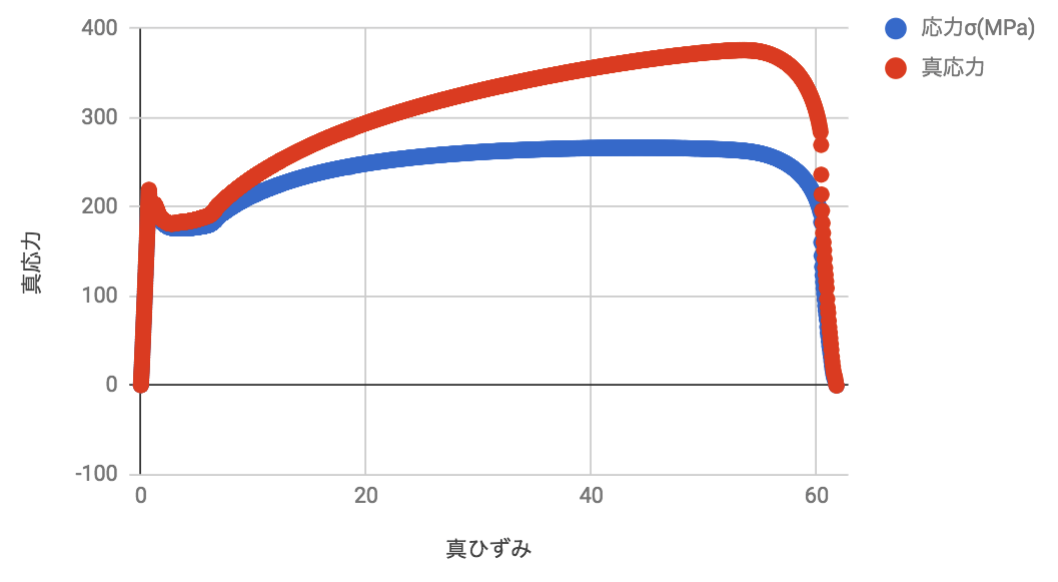
\includegraphics[width=7cm]{../img/spcc_.png}
          \caption{SPCCの公称応力―公称ひずみ線図,真応力―真ひずみ線図}
        \end{center}
      \end{minipage}
      \begin{minipage}{0.5\hsize}
        % 図24
        \begin{center}
          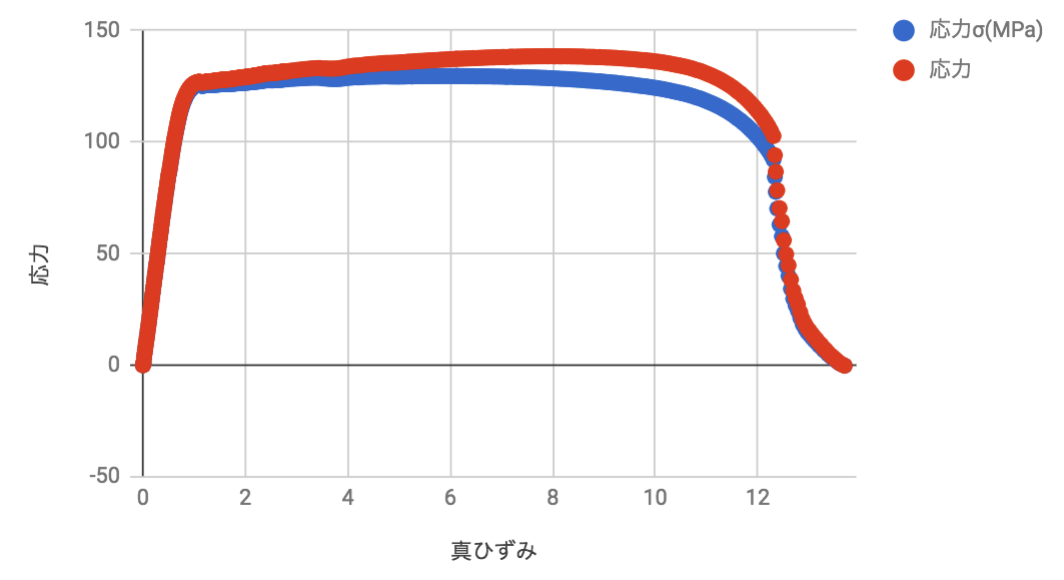
\includegraphics[width=7cm]{../img/a1100_.png}
          \caption{A1100の公称応力―公称ひずみ線図,真応力―真ひずみ線図}
        \end{center}
      \end{minipage}
    \end{figure}

  \subsubsection{各試験片の機械的特性}
  % 各試験片の機械的特性
    SPCC,A1100の縦弾性係数を求めるために用いた真応力―真ひずみ線図を図25,図26に示した.
    また,加えてA1100の0.2\%耐力を求めるため図27に示した.
    さらに,各試験片の機械的特性を表7,8に示した.
      \begin{figure}[htbp]
        % 図25
        \begin{minipage}{0.5\hsize}
          \begin{center}
            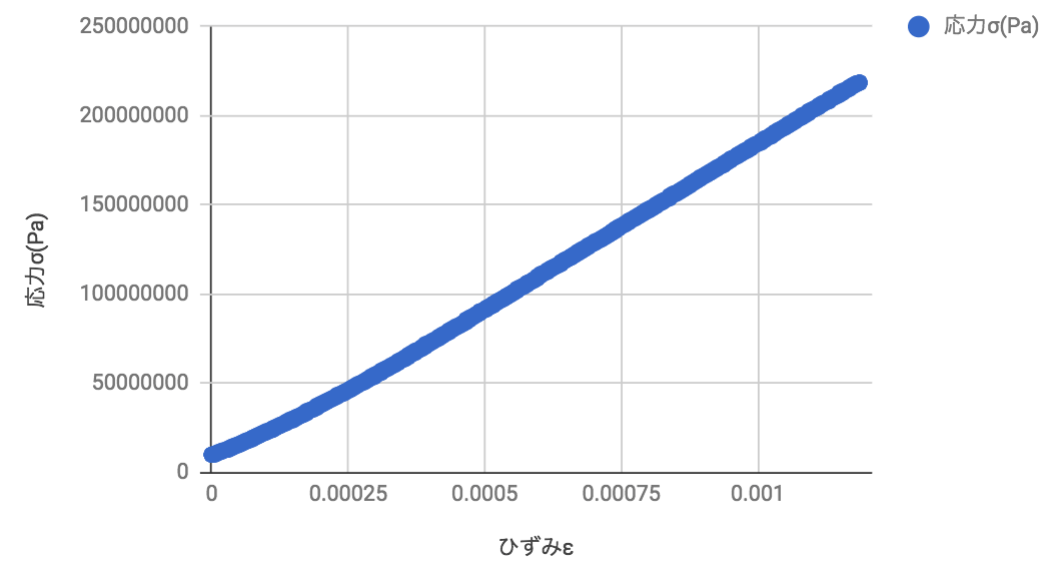
\includegraphics[width=7cm]{../img/spcc_yangu.png}
            \caption{SPCCの真応力―真ひずみ線図}
          \end{center}
        \end{minipage}
        \begin{minipage}{0.5\hsize}
          % 図26
          \begin{center}
            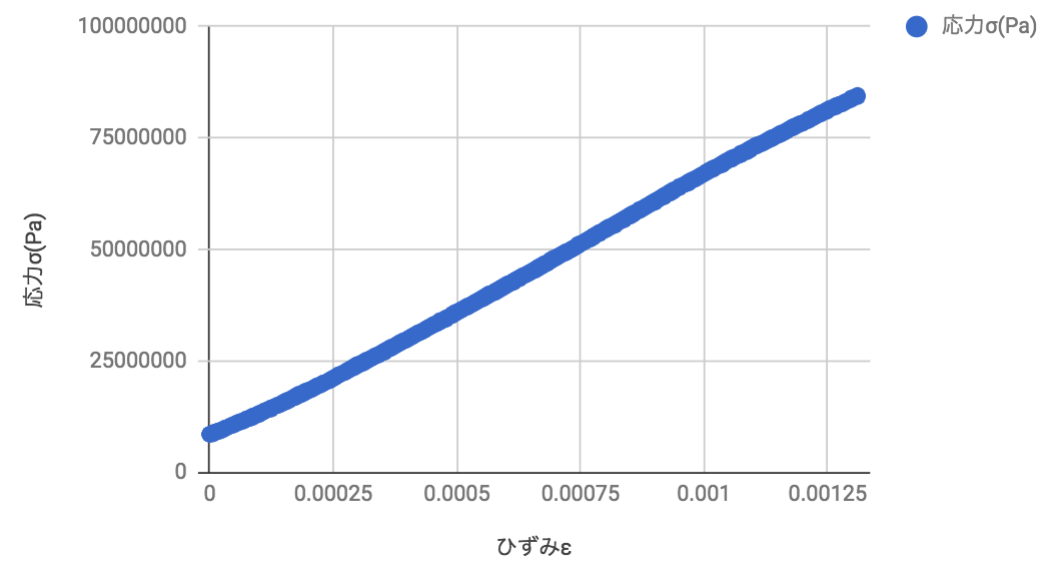
\includegraphics[width=7cm]{../img/a1100_yangu.png}
            \caption{A1100の真応力―真ひずみ線図}
          \end{center}
        \end{minipage}
      \end{figure}
      % 図27
      \begin{figure}[H]
        \begin{center}
          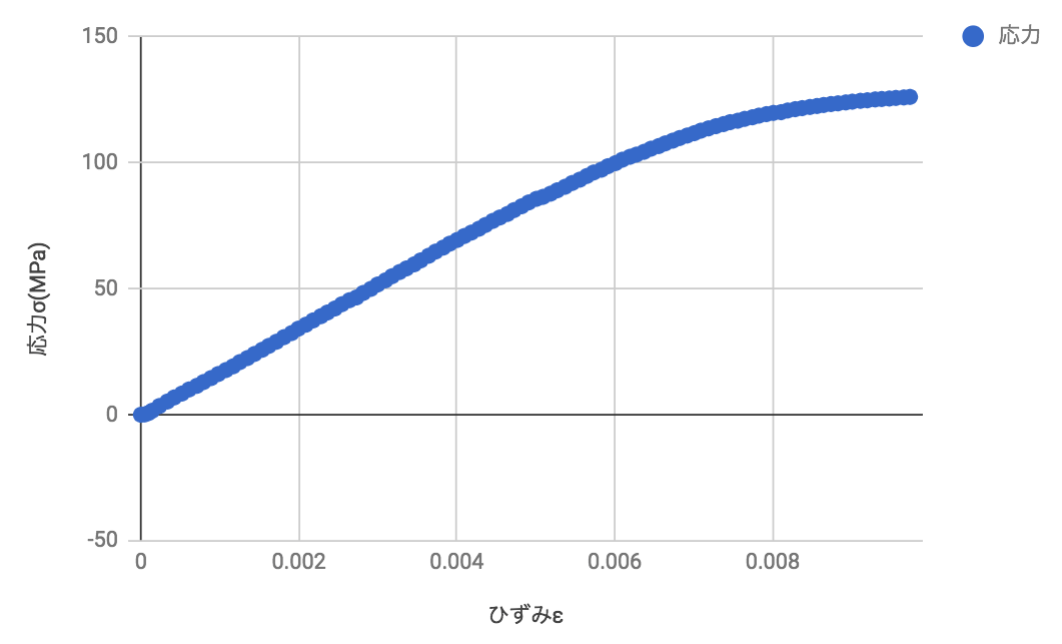
\includegraphics[width=7cm]{../img/zeroni.png}
          \caption{A1100の真応力―真ひずみ線図.0.2\%耐力を計算するために用いた.}
        \end{center}
      \end{figure}
      % 表7
      \begin{table}[H]
        \centering
        \caption{SPCCの機械的特性}
        \label{my-label}
        \footnotesize
        \begin{tabular}{lllllll}
          縦弾性係数(GPa)      & 上降伏点(MPa) & 下降伏点(MPa) & 引張強さ(MPa) & 破断強さ(MPa) & 破断伸び(\%) & 破断絞り(\%) \\ \hline
          $176.7$ & 217.901   & 178.473   & 266.207   & 211.456   & 45\%        & 78\%       
        \end{tabular}
      \end{table}
      % 表8
      \begin{table}[H]
        \centering
        \caption{A1100の機械的特性}
        \label{my-label}
        \footnotesize
        \begin{tabular}{llllll}
          縦弾性係数(GPa)    & 0.2\%耐力(MPa) & 引張強さ(MPa) & 破断強さ(MPa) & 破断伸び(\%) & 破断絞り(\%) \\ \hline
          $57.0$ & 125.319            & 129.706   & 120.364   & 5.5\%        & 71\%       
        \end{tabular}
      \end{table}

\section{考察}
% 考察
  % \subsection{試料No.22 }
  \subsection{極軟鋼,S15C,S45C,SK85,SK105の各組織の観察結果の考察}
  % 極軟鋼
    \subsubsection{(a)試料毎に,熱処理による相変態過程と観察した組織についての説明}
    % a
      \begin{enumerate}
        \item 試料No.22 極軟鋼の焼なまし \\
          炭素をほとんど含まない.なので,温度が$A_{3}$の線を下回るとフェライトのみが析出する.
          図1,2より,フェライトの白い大きな組織が見れた.
        \item 試料No.23 S15Cの焼なまし \\
          炭素の含有率は0.13\%\~0.18\%である.なので,温度が$A_{3}$の線を下回るとフェライトが析出し,
          オーステナイトとフェライトの混合物になる.$A_{1}$の線を下回ると,パーライトとフェライトの混合物になる.
          図3,4より,白いフェライトと黒いパーライトの層状組織が見れた.
        \item 試料No.24 S45C焼なまし \\
          炭素の含有量は0.42\%\~0.48\%である.析出しているものは試料No.23と同じで,温度が$A_{3}$の線を下回ると
          フェライトが析出し,オーステナイトとフェライトの混合物になる.$A_{1}$の線を下回ると
          パーライトとフェライトの混合物になる.しかし,炭素の含有量が多いので,試料No.23よりはパーライトが多かった.
          図3,4ではわかりにくかったが,図7,8を見ると,パーライトは黒と白の縞模様であることがわかった.
        \item 試料No.27 SK85焼なまし \\
          炭素の含有量は0.80\%\~0.90\%である.炭素の含有量が0.80\%のとき,$A_{3}$,$A_{cm}$,$A_{1}$
          の3本の線が交わる.$A_{1}$の線を下回ると,オーステナイトのみからパーライトのみの析出となる.
          図13,14より,パーライトのみが見れた.
        \item 試料No.30 SK105焼なまし \\
          炭素含有量は1.00\%\~1.10\%である.炭素の含有量が0.80\%より多い場合,$A_{cm}$の線を下回ると,
          セメンタイトが析出し,オーステナイトとセメンタイトの混合物となる.$A_{1}$の線を下回ると,
          オーステナイトがパーライトとなり,パーライトとセメンタイトの混合物となる.
          図19,20より,パーライトの組織の間に白い境界線があった.この部分にセメンタイトが析出したと考えられる.  
        \item 試料No.31 SK105焼入れ \\
          焼入れを行うとオーステナイトは急冷された瞬間にマルテンサイトになる.
          図17より,マルテンサイトは針状の物質なことがわかった.
        \item 試料No.32 SK105焼入れ焼もどし \\
          焼入れでマルテンサイトになった後に,焼もどしをすることで,マルテンサイトはソルバイトと
          ルースタイトになる.図21,22より,白と黒色のソルバイトが見れた.
      \end{enumerate}
    \subsubsection{(b)炭素量が,0.03\%→0.15\%→0.45\%→0.85\%→1.05\%のように増加する時の標準組織の変化の説明}
    % b
      手法は焼なましで固定して,試料を変えていった観測結果を表7に示した. 
      \begin{table}[H]
        \centering
        \caption{観測結果から析出した組織をまとめた表}
        \label{my-label}
        \footnotesize
        \begin{tabular}{lll}
          試料No. & 炭素含有量(\%)      & 析出した組織                                                    \\ \hline
          22    & 0.03           & フェライト                                                  \\
          23    & 0.13$\sim$0.18 & \begin{tabular}[c]{@{}l@{}}フェライト\\ パーライト\end{tabular}  \\
          24    & 0.42$\sim$0.48 & \begin{tabular}[c]{@{}l@{}}フェライト\\ パーライト\end{tabular}  \\
          27    & 0.80$\sim$0.90 & パーライト                                                  \\
          30    & 1.00$\sim$1.10 & \begin{tabular}[c]{@{}l@{}}パーライト\\ セメンタイト\end{tabular}
        \end{tabular}
      \end{table}
      炭素の含有量の違いよって,析出する組織も違うと考えられた.(a)の結果と合わせてみると,
      炭素含有量が少ないほどフェライトが,多いほどパーライトが多く析出されたと考えられる.
    \subsubsection{(c)焼入れと焼もどしの目的とマルテンサイト変態,残留オーステナイトについての説明}
    % c
      \begin{enumerate}
        \item 焼入れ \\
          鋼をオーステナイト状態まで加熱した後,水か油に入れて急冷する熱処理であり,
          マルテンサイト組織が析出し,組織を硬いが脆くさせる目的がある.
        \item 焼もどし \\
          焼入れを行なった後の鋼を,100℃\~オーステナイトの生じない温度まで加熱し,空気中でゆっくりと冷却する
          熱処理であり,球状セメンタイトとフェライトで構成されたソルバイト組織が析出し,引張強度や靭性が十分優れた
          鋼にする目的がある.
        \item マルテンサイト変態 \\
          結晶格子中の各原子が拡散を伴わずに協働的に移動することにより新しい結晶構造となる変態である.
        \item 残留オーステナイト \\
          鋼を焼入れする際に,完全にマルテンサイトにはならず,一部未変態のオーステナイトとして残ったものである.
      \end{enumerate}  

  \subsection{SPCC,A1100の引張試験の結果の考察}
  % SPCCの引張試験の結果
    \subsubsection{a}
    % a
      図23,24に示した.
    \subsubsection{b}
    % b
      表7,8に示した.
    \subsubsection{c}
    % c
      SPCCとA1100の機械的特性の違い(縦弾性係数,降伏点,引張強さ,靭性,破断伸び)について比較する.
      \begin{enumerate}
        \item 縦弾性係数 \\
          表7,8よりSPCC,A1100は176,57GPaとなっており,
          同じ寸法の試験片に同じ力を加える場合,縦弾性係数の大きい方が変形しにくい.
          よって,SPCCの方が3.08倍大きいので,より変形しにくい.
        \item 降伏点 \\
          SPCC,A1100は182\~208,121MPaとなっており,
          SPCCの方が大きく,値が小さい方が塑性域に入るまでの力が少ないので,
          SPCCの方が塑性加工しにくい.
        \item 引張強さ,靭性 \\
          SPCC,A1100は277,131MPaとなっており,
          SPCCは約2.1倍大きい.
          靭性は応力―ひずみ線図の図形の面積であり,SPCCの方が大きい.
          これら2点から,強度,靭性においてSPCCの方が優れていた.
        \item 破断伸び \\
          SPCC,A1100は45,5.5\%となっており,SPCCの方が伸びやすい.
        \item まとめ \\
          以上より,炭素鋼はアルミニウムと比較すると,変形しにくく,塑性加工しにくく,
          強度,靭性,延性において優れていた.
      \end{enumerate}
\begin{thebibliography}{3}
  \bibitem{}知能機械工学基礎実験テキスト P.81-P.95
  \bibitem{}矢島悦二郎,若い技術者のための機械・金属材料,丸善出版
  \bibitem{}日本熱処理技術協会,入門・金属材料の組織と性質,大河出版
  \bibitem{}江藤元大他,材料力学,技術堂出版
\end{thebibliography}
\end{document}
\end{document}